\documentclass[]{article}
\usepackage[margin=0.9in]{geometry}

\usepackage{enumitem}
\usepackage{graphicx}
\usepackage{hyperref}
\usepackage{float}
\usepackage{listings}
\usepackage{fancyvrb,newverbs,xcolor}

\lstset{
	language=bash,
	basicstyle=\ttfamily
}

\graphicspath{{images/testing-policy/}{images/logo/}}

\hypersetup{
	colorlinks=true,
	linkcolor=blue,
	filecolor=magenta,
	urlcolor=cyan,
}

%opening
\title{
	\vspace{-1.5cm}
	
\includegraphics[scale=0.7]{docks_round_512.png}
	\\[1cm]
	Testing Policy for Docks
}

\author{\textbf{Team}: TripleParity\\
\textbf{Client}: Compiax\\
\\
\textbf{Team Members}\\
Francois Mentz\\
Connor Armand du Plooy\\
Raymond De Vos\\
Evert Geldenhuys\\
Anna-Marié Helberg\\
Paul Wood}

\date{}

\begin{document}

\maketitle

\tableofcontents
\pagebreak

\section{Testing Process}

\subsection{Peer Review}
Before code can be merged into the develop branch a Pull Request has to be created.
Three reviews are required from other developers before the pull request
can be merged into develop.

During peer reviews the following should be checked:
\begin{itemize}
	\item Architectural problems - will this cause problems in the future?
	\item Compliance with requirements and design - is that what we need?
	\item Coding Standards - proper code formatting and security standards?
\end{itemize}

\begin{figure}[H]
	\centering
	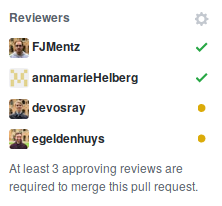
\includegraphics[scale=0.5]{github_3_reviews_required.png}
	\caption{At least 3 peer reviews are needed for a feature to be merged}
\end{figure}

\begin{figure}[H]
	\centering
	
\includegraphics[scale=0.5]{github_approved_review.png}
	\caption{An example of a positive peer review}
\end{figure}

\subsection{Automated Testing and Continuous Integration}
When a commit is made to the 'docks-ui' repository on GitHub two
processes are started:
\begin{itemize}
	\item \href{https://travis-ci.org/TripleParity/docks-ui/branches}{Travis CI} Builds the repository
	\item \href{https://hub.docker.com/r/tripleparity/docks-ui/builds/}{Docker Hub} builds the repository and creates a Docker Image that can be deployed in production
\end{itemize}

\subsubsection{Travis CI}
The history of test reports for Travis CI can be viewed at \url{https://travis-ci.org/TripleParity/docks-ui/branches}.
If the build was not successful it will be marked as 'failed' \\
\\
Travis CI is used for running tests associated with each repository. \\
\\
For the frontend Angular generates a set of tests for each component to verify
that the component was successfully created. These tests run inside a
headless (no screen required) Chrome browser.

The backend also has a suite of unit tests that are executed on Travis CI.

\begin{figure}[H]
	\centering
	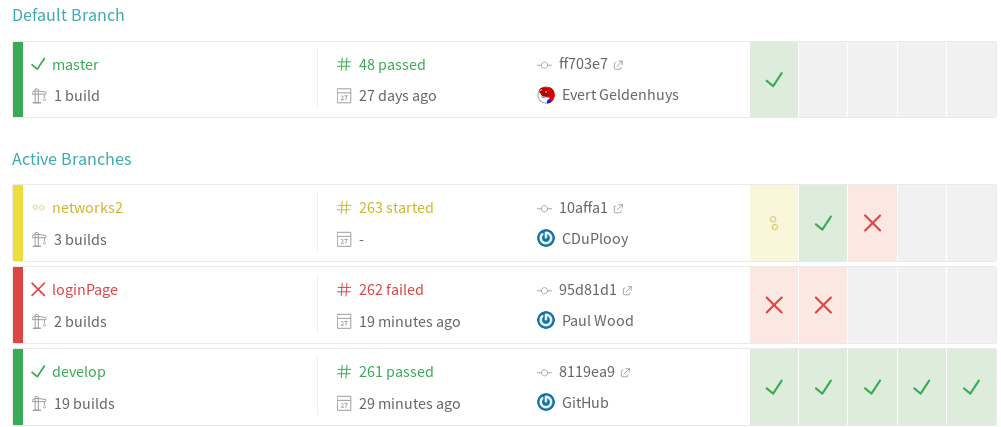
\includegraphics[scale=0.5]{travis_build_history.png}
	\caption{Screenshot of Travis CI branch build history}
\end{figure}

\begin{figure}[H]
	\centering
	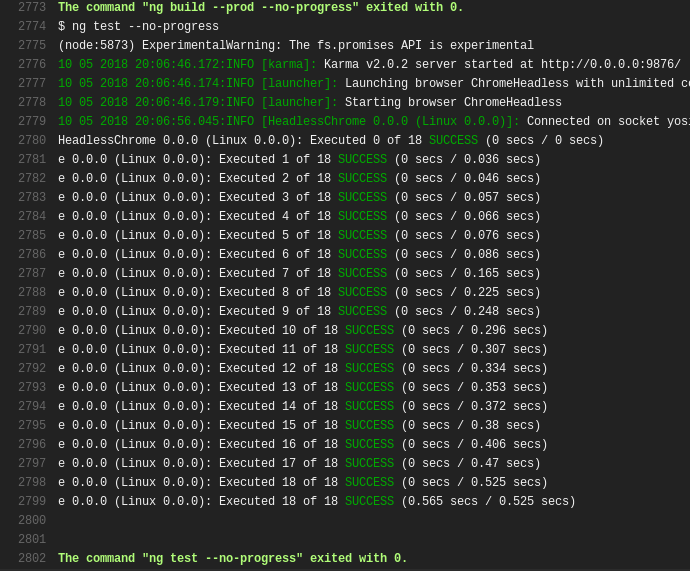
\includegraphics[scale=0.5]{travis_ui_tests_output_1.png}
	\caption{18 UI tests running on Travis}
\end{figure}

\subsubsection{Docker Cloud}
Docker images are build on \href{https://cloud.docker.com/}{Docker Cloud}.
These image can then be deployed in a production environment or for development and testing.
Images can be viewed at \url{https://hub.docker.com/u/tripleparity/}

\begin{figure}[H]
	\centering
	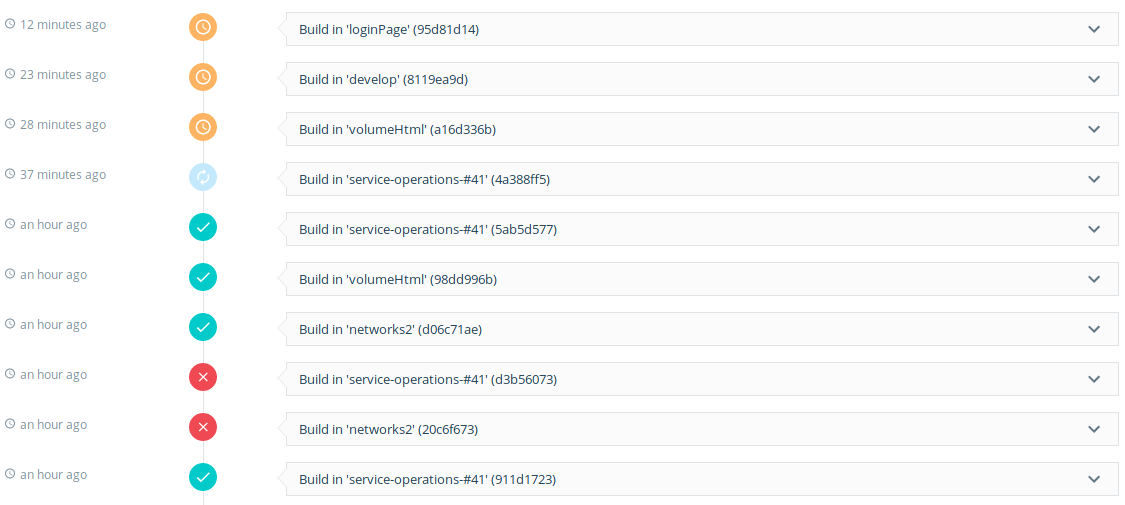
\includegraphics[scale=0.5]{docker_cloud_build_history.png}
	\caption{Screenshot of Docker Cloud Build History}
\end{figure}

\subsection{Docks UI}

\subsubsection{tslint}
Inside of the UI we aditionally use tslint, protractor and karma for testing.
\\
Tslint is a static analysis tool to check typescript code for readability, maintainability and functionality errors.
It can be customised with custom linting rules and formatters.
This can help catch type errors in the code.
\begin{figure}[H]
	\centering
	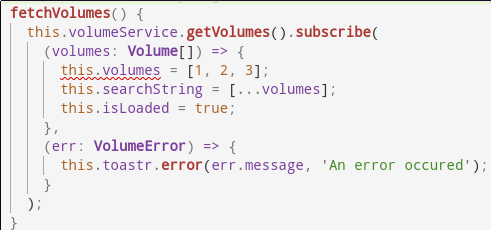
\includegraphics[scale=0.5]{tslint_error.png}
	\caption{Screenshot of tslint linting}
\end{figure}

In the above example an array of numbers is mistakenly assigned to an array of Volumes. 
The linter clearly highlights this as a problem.

\pagebreak

\subsubsection{karma}
Karma is a tool which creates easy testing environments for developers; It's main goal 
is to give developers instant feedback about their test cases.
\begin{figure}[H]
	\centering
	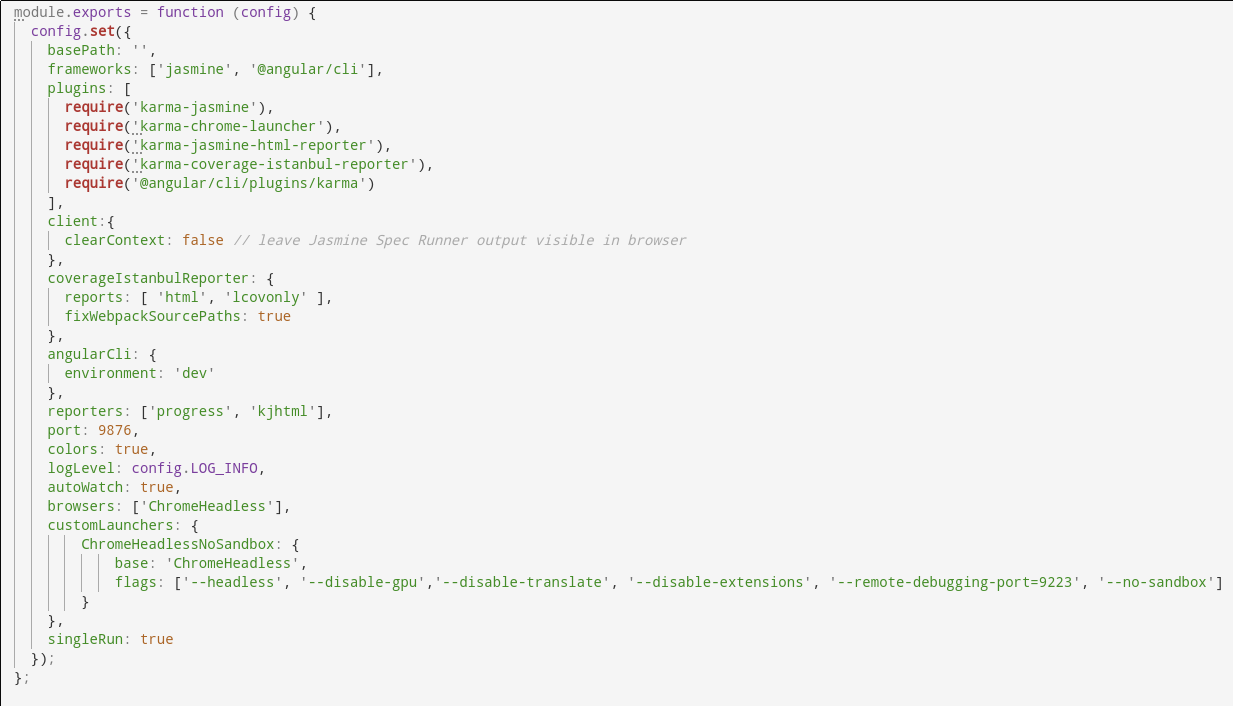
\includegraphics[scale=0.5]{karma.png}
	\caption{Screenshot of karma config}
\end{figure}

In particular we run a headless instance of chrome with all extensions
disabled to test our code; Istanbul is also used to generate a code coverage
report. The test cases are run only once but can be configured such that the tests
are run every time a file is changed.
\\
When a commit is made to a branch, these tests are also run.

\subsubsection{Protractor}
Protractor is an end-to-end test framework. Tests are run in a browser which automatically interacts
with the page as a user would

\subsection{Docks API}

\subsubsection{Eslint}
Eslint is essentially the same as tslint but for javascript.

\subsubsection{Jest}
Jest is a javascript testing framework.
It has some nice features such as instant feedback meaning
failed tests run first. This means we can easily tend to issues.

Jest is used in the backend to run tests on the api itself.
\begin{figure}[H]
	\centering
	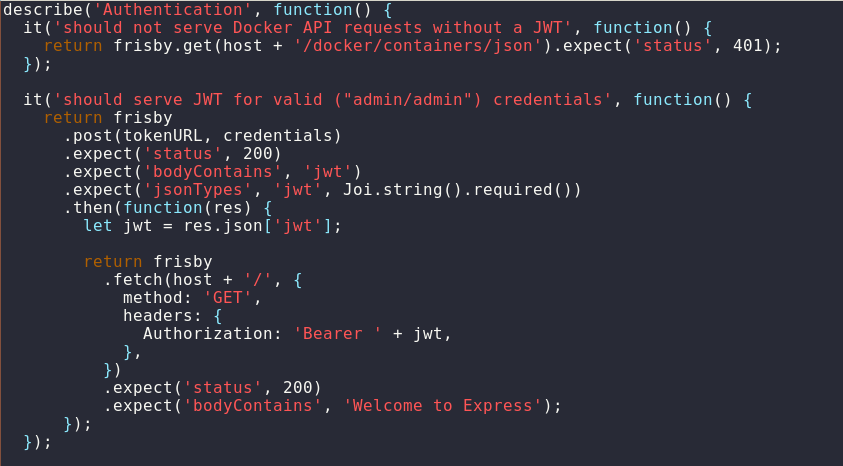
\includegraphics[scale=0.5]{jest.png}
	\caption{Screenshot of jest test}
\end{figure}

\subsubsection{codeclimate}
An automated code review tool.

Tests can be seen \href{https://codeclimate.com/github/TripleParity/docks-ui}{here}.
\begin{figure}[H]
	\centering
	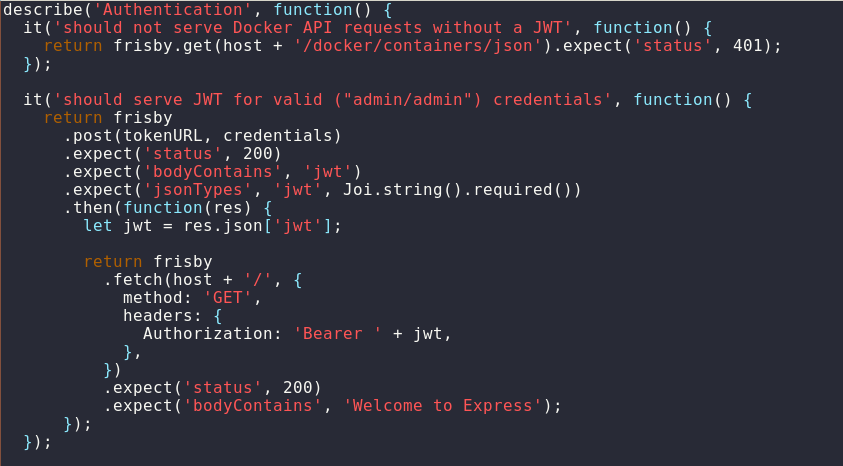
\includegraphics[scale=0.5]{jest.png}
	\caption{Screenshot of codeclimate score}
\end{figure}

\end{document}


